
%=============================================================================%
%=============================================================================%
%=============================================================================%
%=============================================================================%
%=============================================================================%
%=============================================================================%
%=============================================================================%
\section{Overview}
This section discusses many of the foundational concepts leveraged throughout the Power API specification.
It should be noted that many terms commonly used when discussing object oriented languages are used in this section and the document as a whole.
The use of these terms in no way implies that the Power API specification must be implemented using an object oriented language.
%The authors of this specification in fact, recommend the contrary.
We have attempted to achieve two goals, listed in order of priority: 1) programmer portability, where the programmer is the user of the API, and 2) the latitude of the implementor who will often become the user of the API benefitting from our first priority. 

%=============================================================================%
%=============================================================================%
%=============================================================================%
%=============================================================================%
%=============================================================================%
%=============================================================================%
%=============================================================================%
\section{Power API Initialization}\label{sec:PowerAPIInit}


Using any of the Power API interfaces requires initialization. 
Initializaton returns a context.
In the specification, the context is defined as an opaque pointer.
This approach was taken to allow the maximum amount of flexibility to the implementor.
The context returned will contain (act as the entry point to) the system description that is exposed to the user, all policy and privilege information, basically everything the user of the API requires to perform the functionality specified by the API.
The system description is not required to be changed or updated during the life of a specific context.
Initialization is accomplished by calling \funcref{CntxtInit}.
Resources created, like groups, by the user during the life of the context should be cleaned up (destroyed) by the user when no longer needed. 
The implementation is required to clean up all context resources when the user calls \funcref{CntxtDestroy}.

%=============================================================================%
%=============================================================================%
%=============================================================================%
%=============================================================================%
%=============================================================================%
%=============================================================================%
%=============================================================================%
\section{Roles}\label{sec:Roles}

The Power API specification leverages the concept of Roles. 
Roles represent the different types of users that exist which include:
\begin{itemize}[noitemsep,nolistsep] %
\item{\textbf{Application}  The application or application library executing on the compute resource. May also include run-time components running in user space.}
\item{\textbf{Monitor and Control}  Cluster management or Reliability Availability and Serviceability (RAS) systems, for example.}
\item{\textbf{Operating System} Linux or specialized Light Weight Kernels which are found on HPC platforms and potentially portions of run-time systems. }
\item{\textbf{User} The user of the HPC platform. }
\item{\textbf{Resource Manager} This can include work load managers, schedulers, allocators and even portions of run-time systems. }
\item{\textbf{Administrator} The system administrator or HPC platform manager. }
\item{\textbf{HPCS Manager} The individual or individuals responsible for managing policy for the HPC platform, for example. }
\item{\textbf{Accounting} Individual or software that produces reports of metrics for the HPC platform. }
\end{itemize}
These brief definitions are not meant to be exhaustive.
Roles are analogous with the \textit{Actors} discussed in section \ref{sec:UseCase}.
In some cases roles become the system that other roles interact with.
For example, we specify an interface between the Application role (HPCS Application in figure \ref{fig:UCDTopLevel}) and the Operating System (HPCS Operating System in figure \ref{fig:UCDTopLevel}).
The Operating System is the system (in UML terminology) that the Application role is interacting with. 
Notice in figure \ref{fig:UCDTopLevel} that the specification also includes an interface between the Operating System role and the Hardware (HPCS Hardware in figure \ref{fig:UCDTopLevel}).
These and other interfaces are described in chapter \ref{chap:Interfaces}.
The user of the API is required to specify what role they will assume when interacting with the system upon initialization of the API.

%The implementation is required to associate an integer precedence with each role, zero (0) being the highest precedence.
%Roles may have the same precedence number which indicates the roles have equal precedence.
%Other factors, such as user name and permissions can be used to make precedence determinations at finer granularity.
%This feature is provided as a mechanism for the implementation to determine which operation has priority especially in cases where operations conflict.

%For example, the Administrator role (assigned precedence 0) sets a power cap for node 0 at 200W. 
%The Resource Manager role (assigned precedence 1) would like to manage the power cap for an application which uses a number of nodes including node 0.
%The Application role (assigned precedence 2) would like to fine tune the power cap of one of the nodes it is executing on (node 0). 
%The implementation can use the precedence numbers in a variety of ways given the assumptions above.
%In this scenario, the Administrator role is allowed to set the power cap for node 0 at 200W.
%If the Resource Manager requests a power cap of 210W for node 0 the operation would be denied given a role with higher precedence requested a lower power cap.
%If the Resource Manager requests a power cap of 180W for node 0, the operation is allowed.
%Likewise the Application role is permitted to request a lower power cap for node 0 but not a higher power cap.
%First note, the specification does not proscribe these rules, it only provides the precedence mechanism as a way to implement them.
%Also note, this example could be accomplished by simply determining precedence based on which role is requesting the operation.
%The precedence concept is provided in cases where, for example, the implementation requires two roles to have equal precedence.
%If we add to the above scenario the Operating System role (precedence 0), the Operating System has the ability to request that the power cap for node 0 be raised to 210W.
%Once more the specification is not proscribing this rule, only illustrating the need for an additional mechanism that can be used by the implementation to enforce similar scenarios.
%
%\laros{Add a reference here for the call that can be used to get the implementation assigned precedence numbers for each role.}

Roles are also provided as a mechanism for the implementation to express priority or precedence in circumstances where, for example, conflicting operations are requested. 
%More detail on this topic is provided in section \ref{sec:Initialization} (Initialization).


%=============================================================================%
%=============================================================================%
%=============================================================================%
%=============================================================================%
%=============================================================================%
%=============================================================================%
%=============================================================================%
\section{System Description}\label{sec:PowerAPIBaseSysDesc}

\begin{figure}
	\begin{center}
		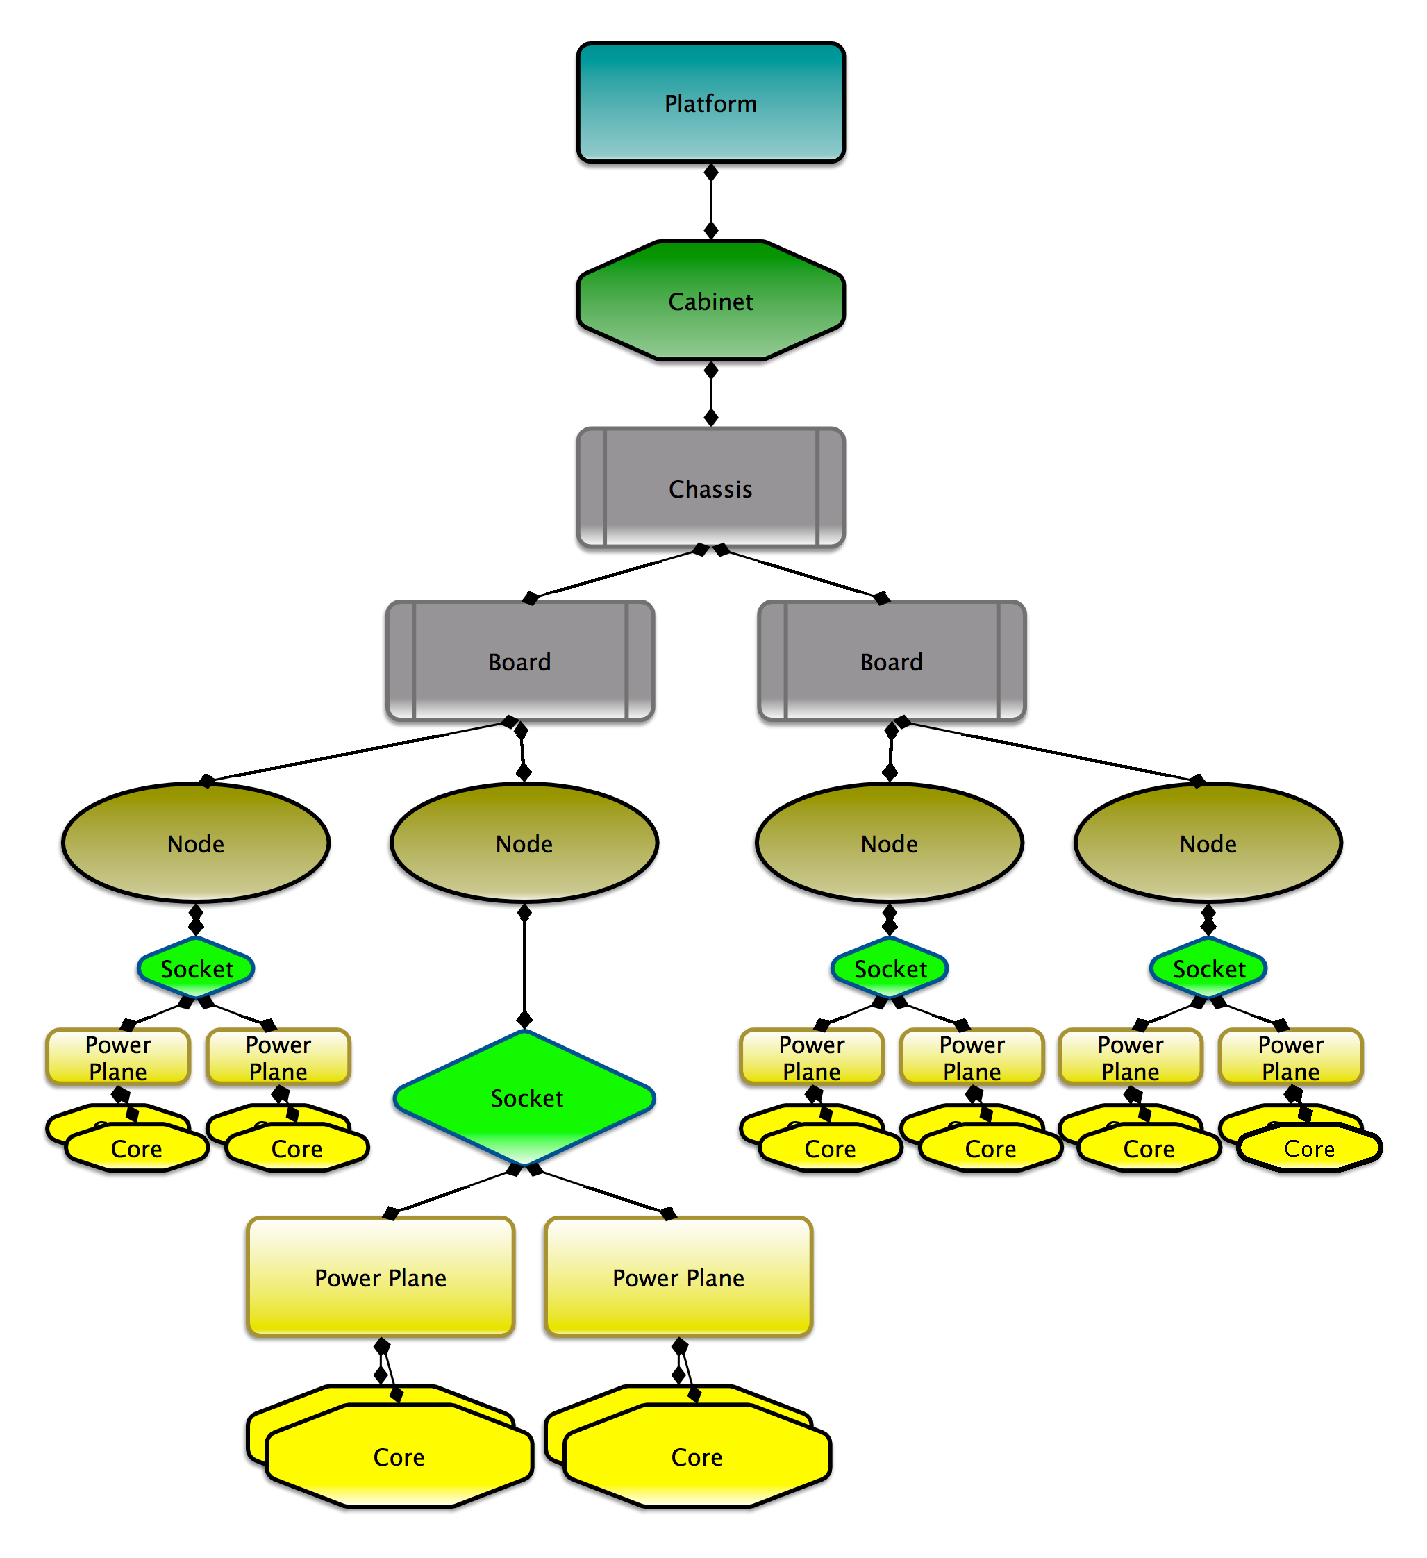
\includegraphics[width=0.80\linewidth,height=.60\paperheight]{FIGURES/PowerAPIMachineHierarchy5dot1}
	\end{center}
	\caption{Hierarchical Depiction of System Objects}
	\label{fig:BaseSystemMap}
\end{figure}

The system description is the \textit{view} of the system exposed to the user upon initialization via the context that is returned.
Figure \ref{fig:BaseSystemMap} depicts an example of a system description showing a hierarchical arrangement of objects.
All object types listed in the specification must be defined by any implementation, but do not have to be used in the system description.
The implementation chooses which objects will be employed in the system description and how they will be arranged.
An object can only have a single parent but may have multiple children.
Currently, a system description may only describe a single platform and have a single object of type \texttt{Platform} which represents the top of the hierarchy. 
Later revisions of the specification may include the ability to combine multiple platforms in the system description. 
This might be useful, for example, in representing an entire datacenter. 
While figure \ref{fig:BaseSystemMap} depicts a homogeneous system description, homogeneity is \textit{not} a requirement. 
In practice a system description can be heterogeneous and unbalanced.

To summarize the requirements:
\begin{itemize}[noitemsep,nolistsep] %
	\item{
	The \texttt{Platform} object type must be defined by the implementation and must appear at the top of the system description.
	}
	\item{
	All object types in this specification must be defined in any implementation. The use of the object types, with the exception of the \texttt{Platform} object type, is optional.
	}
	\item{
	Objects can only have one parent but may have many children. Currently the \texttt{Platform} object has no parent since it appears at the top of the system description. This will likely change in future versions of the specification.
	}
        \item{
        If an implementation chooses to add objects not defined in the specification they should only be exposed to the user in a vendor specific context to avoid unpredictable or non-portable behaviour (see \funcref{CntxtInit}).
        }
\end{itemize}

%Figure \ref{fig:BaseSystemMap} depicts a hierarchical arrangement of all of the  platform objects that must be included (defined) in any implementation of the API.
%In addition to the requirement that these object types must be defined in any implementation, they also must be organized in the order shown in figure \ref{fig:BaseSystemMap}.
%For example, an implementation must always position objects of type \textit{Cabinet} under the top level \textit{Platform} object.
%Likewise, objects of type \textit{Board} must appear below an object of type \textit{Cabinet}.
%There can only be a single object of type \textit{Platform}, and that object must be the top of the hierarchy.

The following is a list of the object types currently included in the specification along with a short description of each.
\begin{itemize}[noitemsep,nolistsep] %
	\item{
Platform - Currently, the one and only Platform object is the top level object of the system description exposed to the user of the API. 
The Platform object is intended to conceptually represent the entire Platform.
For example, if the Platform object has a power or energy measurement or control capability exposed through the Platform objects attributes the scope of these attributes should be platform wide.
}
	\item{
Cabinet - Objects of type Cabinet are intended to represent the cabinets or racks that act as enclosures (or logical groupings) for the platform equipment. 
Beyond the utility of convenient groups of lower level objects (equipment) cabinets may have power or energy relevant capabilities which can be exposed through attributes associated with each Cabinet object. 
}
	\item{
Chassis - Objects of type Chassis are intended to be used for finer grained organization of objects within the higher level Cabinet object. Chassis, like cabinets may have power or energy relevant capabilities that can be exposed to the user.
}
	\item{
Board - Board objects offer another method of organization for underlying objects (equipment). 
Boards may also have power and or energy relevant capabilities which can be exposed through associated attributes. 
For example, a board could contain the power supply and the point of instrumentation for collecting power or energy samples for a node or multiple nodes.
}
	\item{
Node - The Node type is probably one of the most universally important object types. 
Measuring and controlling the power and or energy characteristics of a node or multiple nodes (grouped into multiple Boards, Chassis or Cabinets) is important for a many reasons and provides a wide range of flexibility of configuration to the implementor. 
For example, on HPC platforms a single application typically executes on many nodes. 
Understanding the energy use of an application run can be obtained by collecting the energy use (via the appropriate Node attribute) for each node participating in that application execution. 
Node objects will likely have many attributes exposing many power and energy relevant capabilities.
}
	\item{
Socket - The Socket object is intended to represent the one or more processor sockets, or other component types that can be thought of as sockets, that make up a Node. 
For example, a single Node object may be a dual socket (dual CPU) node.
The implementor may choose to enclose other component types (a NIC for example) within a Socket object, or add other object types as they see fit to represent the architecture they are describing.
They can also decide to omit the use of this, or any other object type (currently other than Platform) in the system description.
}
	\item{
Power Plane - The Power Plane object is used to organize lower level objects (any types of objects) within a power domain or single point of measurement and or control.
For example, a pair of cores may share a power plane within a socket. 
This configuration is depicted in figure \ref{fig:BaseSystemMap}. 
This organization allows a pair of cores to be controlled from a single power control point in the hierarchy for convenience. 
This object type allows these power and energy relevant relationships to be expressed anywhere in the system description.
}
	\item{
Core - Core objects are intended to represent the individual processor cores within multi-core CPUs (or possibly GPUs). 
Modern architectures have an increasing number of cores per CPU (or GPU). 
In the near future it is likely that an abstraction between Socket and core would become useful as the number of cores increase. 
Physical and logical groupings of cores already exist in current architectures.
}
	\item{Memory - The Memory object type is included to represent the growing range of memory types that exist on HPC platforms. 
Individual cores, for example, have Memory in the form of cache which the implementor may choose to organize differently from the main memory of the Node or a tertiary level of memory such as NVRAM.
}	
	\item{
NIC - The NIC object is intended to represent the Network Interface Controller.
As with many other object types, the organization of a NIC in relation to Boards, Nodes or even Cores is architecture dependent.
The NIC object type is included in hopes that there are power and energy relevant capabilities included in future NICs.
}	
        \item{
HT - The HT (Hardware Thread) object represents an OS-visible CPU.  
While from a physical perspective frequency and voltage changes occur at the physical core level, it is usually the case that these must be configured by software at the OS-visible CPU level.  
Typically the lowest-common denominator among all OS-visible CPUs is used to configure the physical core.
}

\end{itemize}

Additional object types may be defined by the implementor and placed anywhere in the hierarchy as long as the previously stated rules are not violated.
Ultimately, the  object types defined in this specification, and those added by the implementor, will be used to produce a system description describing the system presented to the user via the context returned upon initialization.
Objects are used as interfaces to underlying functionality.
The specification does not assume state is retained for objects.
Additionally, the specification makes no guarantees with regards to race conditions between processes or threads.

%=============================================================================%
%=============================================================================%
%=============================================================================%
%=============================================================================%
%=============================================================================%
%=============================================================================%
%=============================================================================%
\section{Attributes}\label{sec:TheoryAttributes}
Attributes are an important part of the Power API.
A large amount of basic functionality is exposed through the use of attributes.
The term attribute is used somewhat conceptually since some attributes are implicit while others are explicitly defined as part of a required specification data structure (page \pageref{type:AttrName}).
Attributes are used for a number of reasons such as to navigate through the system description, to access information or a measurement (sensor information for example) and for control (setting a P-state for example).
Global attributes are attributes that are present for every object defined; whether required by the specification or added by the implementor. 

The following is the list of global attributes:
\begin{itemize}[noitemsep,nolistsep] %
\item{name} - Unique identifying name of the object (see \funcref{ObjGetName}).
\item{entry point} - The position in the hierarchy after initialization (see \funcref{CntxtGetEntryPoint}).
\item{type} - The type of the object (see \funcref{ObjGetType}).
\item{parent} - The parent of an object is the object that is above it in the hierarchy (see \funcref{ObjGetParent}).  The only exception is the currently single platform object whose parent is a pointer to NULL. 
\item{children} -  Object or objects directly below an object in the hierarchy (see \funcref{ObjGetChildren}).
\end{itemize}

Note, in the list above all the attributes are implicit. 
Explicit attributes are defined in the \typeref{AttrName} type definition.
The majority of the attributes defined in the specification, and likely those added by an implementator, are, and will be, explicit.
The implicit attributes defined above are primarily used for navigation and are accessed through attribute specific functions which are described in Section \ref{sec:Navigation}.

Explicit attributes are either accessed through the generic attribute interface (Section \ref{sec:Attributes}) or attribute specific functions found in either the section describing the specific interface in which they are used or in Chapter \ref{chap:Common}, \textit{Core (Common) Interface Functions}.

The attribute interface is intended to keep the specification from growing every time additional functionality is either specified or added by an implementor. 
As long as the new functionality fits within the defined attribute interfaces no additional API functions are required to be specified.

%=============================================================================%
%=============================================================================%
%=============================================================================%
%=============================================================================%
%=============================================================================%
%=============================================================================%
%=============================================================================%
\section{Metadata}\label{sec:TheoryMetadata}
Each object and object attribute pair can have additional descriptive metadata associated with it.
This information is often useful for getting a better understanding of the meaning of objects and attributes and how to interpret the values read from attributes.
Examples include a human readable name and description strings, the list of values supported by an attribute, and measurement accuracy and precision.
The metadata interface (see section \ref{sec:METADATA}) returns information relevant to either a specific object or a specific attribute of a specific object.
A given attribute name may have different metadata for different objects, even if the objects are of the same type (e.g., the voltage attribute of two node objects may have different metadata accuracy values).


\section{Thread Safety}\label{sec:ThreadSafety}
Implementations of the Power API are not required to provide thread safety to multiple threads of the same process.  
If necessary, users of the Power API must use locking or some other mechanism to ensure that only one thread per process calls into the Power API at a time.  
This requirement only applies to threads of the same process that may issue conflicting operations.  
Different processes may make simultaneous Power API calls without any coordination.  
If thread concurrency within a process is required, the \funcref{CntxtInit} function can be called multiple times to initialize multiple Power API contexts.  
Multiple threads of the same process may then simultaneously call into the Power API, so long as each thread operates on a different Power API context.  
For example, a process with four threads may create four Power API contexts and associate one context with each thread.  
The threads may then make Power API calls without any additional coordination, so long as each thread operates only on its assigned context and the objects exposed by its assigned context. 
Threads should not operate on objects exposed by another thread's context without employing locking or some other coordination mechanism.

